%!TEX root = /Users/smsohan/Taggy/Thesis/ucalgthes1_root_0.tex
\fancyhead[RO,LE]{\thepage}
\fancyfoot{} 
\chapter{QUANTITATIVE EVALUATION}
\label{ch:evaluation}
As mentioned in the research goals, an evaluation is required to measure the accuracy of Taggy in auto-tagging emails with user stories. In this thesis, the evaluation is based on two different real world data sets, collected from two different sources. In total the data represents A agile teams' work across X iterations comprising a total Y days. The evaluation shows that for different projects Taggy can correctly auto-tag between 76 to 80\% emails with user stories after sufficient training.

This chapter is organized as follows: Firstly, the evaluation approach is discussed. As a part of it, the adapted definition of accuracy is given. Next, a null hypothesis is stated which is used in deducing the statistical relevance of the evaluation results. Then, the two data sets are described and the evaluation results for each are provided in detail. Finally, the limitations of this evaluation are discussed.

\section{Evaluation Approach}
The evaluation steps, as depicted in Figure~\ref{fig:evaluation}, are described below.

\begin{figure*}[tb]
	\centering
	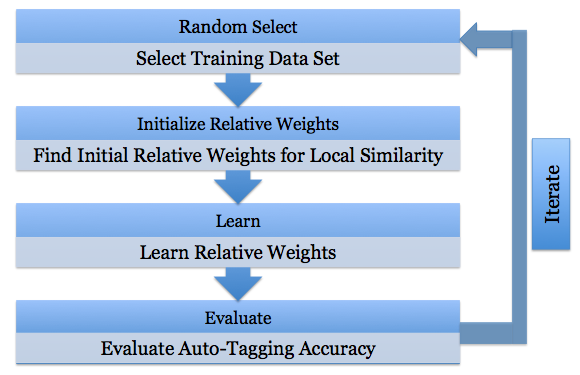
\includegraphics[width=\textwidth]{Evaluation.png}
    \caption{Taggy Empirical Evaluation Steps}
	\label{fig:evaluation}
\end{figure*}


\begin{enumerate}
	\item \textbf{Random Select.} Randomly select 10\% emails from all available emails for training. Training emails are randomly selected to improve the possibility of encountering different patterns in the data.
	\item \textbf{Initialize Relative Weights.} Initialize the relative weights for temporal, people, subject and body similarities using the training data from step\# 1.
	\item \textbf{Learn.} Use the reward-punishment approach for each training email from step\# 1, adjust the relative weights.
	\item \textbf{Evaluate.} Using the adjusted relative weights from step\#3, auto-tag the remaining emails that were not included in the training data in step\# 1. This ensures the training data and evaluation data contain completely disjoint sets of emails. Compute the accuracy of the auto-tagging.
	\item \textbf{Iterate.} Repeat steps 1 to 4, with 20\%, 30\%, 40\% and 50\% data for training. This step attempts to find an optimum partition of  training data set where the relative weights converge to a point so that adding more training data adds little value to the auto-tagging accuracy.
	
\end{enumerate}

\subsection{Accuracy}
The accuracy of auto-tagging is a ratio between the number of correct tags and the total number of emails presented for evaluation. Since this excludes the training data set, the accuracy only represents the accuracy over the evaluation data set. So, the accuracy is computed using Equation~\ref{eq:accuracy}.
	
\begin{equation}
\label{eq:accuracy}
Accuracy = \frac{Number \;  of  \; correct  \; auto tagging} {Number \;  of \;  total \;  evaluation \;  emails }  \; *  \; 100  \; \%
\end{equation}
	
As Equation~\ref{eq:accuracy} suggests, it is necessary to be able to justify whether an auto-tagging is correct or incorrect. So, the evaluation data needs to provide information about correct relationship of an email with user stories so that the auto-tagged results can be compared against  known values.

\subsection{Statistical Relevance}
The statistical relevance is found by starting with a null hypothesis and then refuting it based on chi-square test. In this case the null hypothesis is:

\begin{quote}
	The auto-tagging accuracy of Taggy is no better than a random decision making.
\end{quote}

The outcome of an auto-tagging process is either a correct or a wrong tagging of an email against the user stories in a project. Similarly, a random system will produce one of the two outcomes. The target of this statistical relevance determination is to see if the accuracy found from Taggy's evaluation is likely to be achievable by a random system.

In this case, we have a single degree of freedom, since there are two possible outcomes, correct and wrong. And the expected value of correct and wrong is same for a random system. Based on this information, the chi-square computation is done using Equation~\ref{eq:chi}:



\begin{equation}
\label{eq:chi}
\begin{split}
	\chi ^ 2 = \frac {(Count \; of \; correct \; tagging \; - \; half \; of \; total \; evaluation \; emails) ^ 2} {half of total evaluation emails} +  	
\\
	\frac{(Count \; of \; wrong \; tagging \; - \; half \; of \; total \; evaluation \; emails)  ^ 2} {half \; of \; total \; evaluation \; emails}
\end{split}	
\end{equation}                                       

This computed value is compared against the upper critical chi-square value for probability 0.05 with 1 degree of freedom, that is $\chi^{2}_{0.05}$=3.841. The probability value of 0.05 is conventionally used in significance finding. A value beyond this threshold indicates disagreement between the observation and the null hypothesis. We also present the corresponding p-values against the computed chi-square values. The lower the p-value, the less likely is the observation given the null hypothesis is true.

\section{Evaluation Results}
The evaluation results are discussed in two sections for two different data sets.

\subsection{Data set\# 1: ScrumPad}	
This data set was obtained from the online agile project management tool called ScrumPad.	ScrumPad allows users to manage product backlog, perform iteration planning and track progress. Also, it lets users discuss the project's user stories using message threads. Each message thread can contain an explicit link to a user story. While sending a message using ScrumPad, one can link it with a user story. The messages are stored in ScrumPad database and also sent to people via emails. People can directly reply to the notification emails, which goes to ScrumPad and gets saved as a message of an existing thread.

The user stories in ScrumPad contain information about its title, description, attachments, customer, developers and iteration. Taggy used these user stories to train and evaluate its auto-tagging performance.

The messages in the ScrumPad message threads are treated as emails for the evaluation of Taggy. Messages contain subject, body, sender, recipients and attachments. These fields are mapped against the fields of emails. Also, if a message thread in ScrumPad is linked against a user story, all derived emails from the messages of that thread are also treated to be linked against the user story. So, these are essentially the correct taggings for the emails since they were all manually provided by the contributors to the message threads. This information helps the training of Taggy using reward-punishment approach with the necessary feedback. Also, the accuracy computation relies on this information to find if an auto-tagging is correct or not.

The ScrumPad data set contains data from five distributed agile projects. Four of the five projects, MethodMarketing, BI for Car Dealers, ManyWheels and VarsityDays were developed by Code71, Inc. (www.Code71.com). Code71 is also the creator of ScrumPad. These four projects employed developers from Dhaka, Bangladesh and Virginia, USA. These projects were developed for four different clients from the USA.

The fifth project, MindAndMarket, was distributed among one developer from Bangladesh, and two developers and a client from Belgium. The Belgian development team and the client worked at the same city.

\begin{table}
	\label{tab:scrumpad}
  \centering
  \caption{Scrumpad Data Set}
    \begin{tabular}{|p{2cm}|p{4cm}|r|p{1cm}|p{1.2cm}|p{1.2cm}|r|}
      \hline
      \textbf{Project Name} & \textbf{Description} & \textbf{Users} & \textbf{Itera- tions} & \textbf{It. Len. (days)}  & \textbf{User Stories} & \textbf{Emails}\\
      \hline
      Method Marketing & Online loan application & 7 & 14 & 14 & 86 & 183 \\
      \hline
      BI for Car Dealers & A decision support tool for vehicle dealers & 7 & 11 & 14 & 70 & 213 \\
      \hline
      Many Wheels & A web application for transporters and shippers & 5 & 12 & 14 & 97 & 158 \\
      \hline
      Varsity Days & A social networking application for school sports teams & 5 & 15 & 14 & 88 & 46 \\
      \hline
      Mind And Market & A project collaboration tool & 3 & 6 & 7 & 28 & 40 \\
      \hline
      \textbf{Total} &  &  &  &  & \textbf{369} & \textbf{640}\\
      \hline
      \multicolumn{7}{l}{Source: \emph{www.ScrumPad.com}}
    \end{tabular}
\end{table}

Table~\ref{tab:scrumpad} shows the composition of this data set. It is worth mentioning that the emails here are the ones that were exchanged using ScrumPad. So, the actual numbers of emails in these projects are not limited to the numbers as mentioned in the table.

\begin{figure*}[htb]
	\centering
	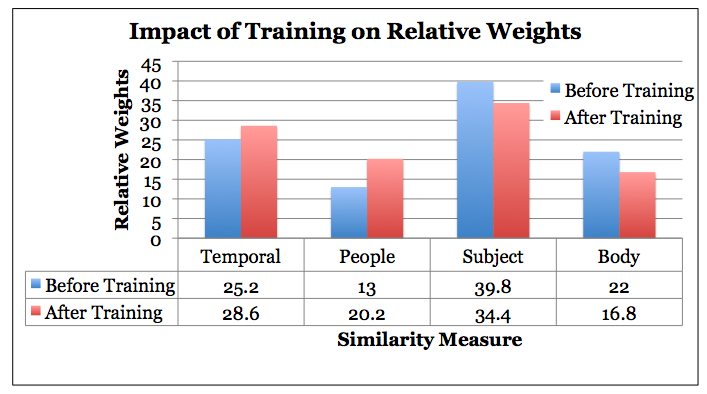
\includegraphics[width=\textwidth]{training.png}
    \caption{Impact of Training on Relative Weights}
	\label{fig:training}
\end{figure*}

Given this data, the aforementioned evaluation approach was followed to train and auto-tag the emails. The iterative approach in finding an optimum size of the training data set partition yielded 20\% of the total data. So, with a random partition containing 20\% of all emails for training produced better auto-tagging accuracy than a smaller sized partition and was as good as a larger sized partition. Chart~\ref{fig:training} shows the impact of training on the relative weights of different similarity measures. The chart shows that the initial relative weights for the similarity measures of the text components are reduced while the context components are increased as a result of the training.

The maximum similarity score for a local similarity measure can be 1 as shown in the similarity equations before. Using the trained relative weight values and a threshold global similarity score of 0.58, an email will be auto-tagged with a user story if one of the following is true:
\begin{enumerate}
	\item The email has strong text similarity (maximum 0.34 + 0.17 ~= 0.51) and some context similarity with the user story.
	\item The email has context similarity (maximum 0.29 + 0.20 ~= 0.49) and some text similarity with the user story.
\end{enumerate}
So, setting such a threshold score forces auto-tagging decisions to be based on both context and text relevance. This threshold was found from observing the data as in most cases when an email is actually related to a user story, their global similarity score was computed greater than or equal to 0.60. The trade-off between selecting this threshold and auto-tagging is discussed later in Chapter~\ref{ch:discussion}.

Using this threshold and the trained relative weights, the evaluation yielded the results as shown in Table~\ref{tab:sp_evaluation}.

\begin{table}
	\label{tab:sp_evaluation}
  \centering
  \caption{Evaluation Using Scrumpad Data Set}
    \begin{tabular}{|p{2cm}|p{2cm}|p{2cm}|p{2cm}|p{2cm}|p{2cm}|p{2cm}|}
      \hline
      \textbf{Project Name} & \textbf{Total Emails} & \textbf{Training Emails (20\%) of Total} & \textbf{Evaluation Emails (80\%)  of Total} & \textbf{Correct Auto-Tagging} & \textbf{Accuracy} & $\chi^{2}$\\
      \hline
      Method Marketing & 183 		& 37	& 146	&	111 & \textbf{76\%}	& 39.6\\
      \hline
      BI for Car Dealers & 213 	& 43	& 170	&	133	& \textbf{78\%}	& 54.2\\
      \hline
      Many Wheels & 158 				& 32	& 126	& 93	& \textbf{74\%}	& 28.6\\
      \hline
      Varsity Days & 46 				& 9		&	37	& 29	& \textbf{79\%}	& 12\\
      \hline
      Mind And Market & 40 			& 8		& 32	&	24	& \textbf{74\%}	& 8\\
      \hline
      \textbf{Total} & 640 			& 129	& 511	&	390	& \textbf{76\%}	& 141.6\\
      \hline
      \multicolumn{5}{l}{Source: \emph{primary}}
    \end{tabular}
\end{table}

As shown in Table~\ref{tab:sp_evaluation}, out of a total of 511 evaluation emails, Taggy could produce correct auto-tagging of 390 emails. This result is found after using 129 emails for training. The training data was selected randomly from the five projects. The table also shows that the $\chi^{2}$ values are greater than single degree of freedom $\chi^{2}_{0.05} = 3.841$, which refutes the null hypothesis as stated before.



\subsection{Data set\# 2: IBM Jazz Rational Team Concert}
\section{Limitations}
	
